\section{Discussion and limitations of our analysis}

\begin{figure*}
\begin{center}
    \begin{tabular}{cc}
    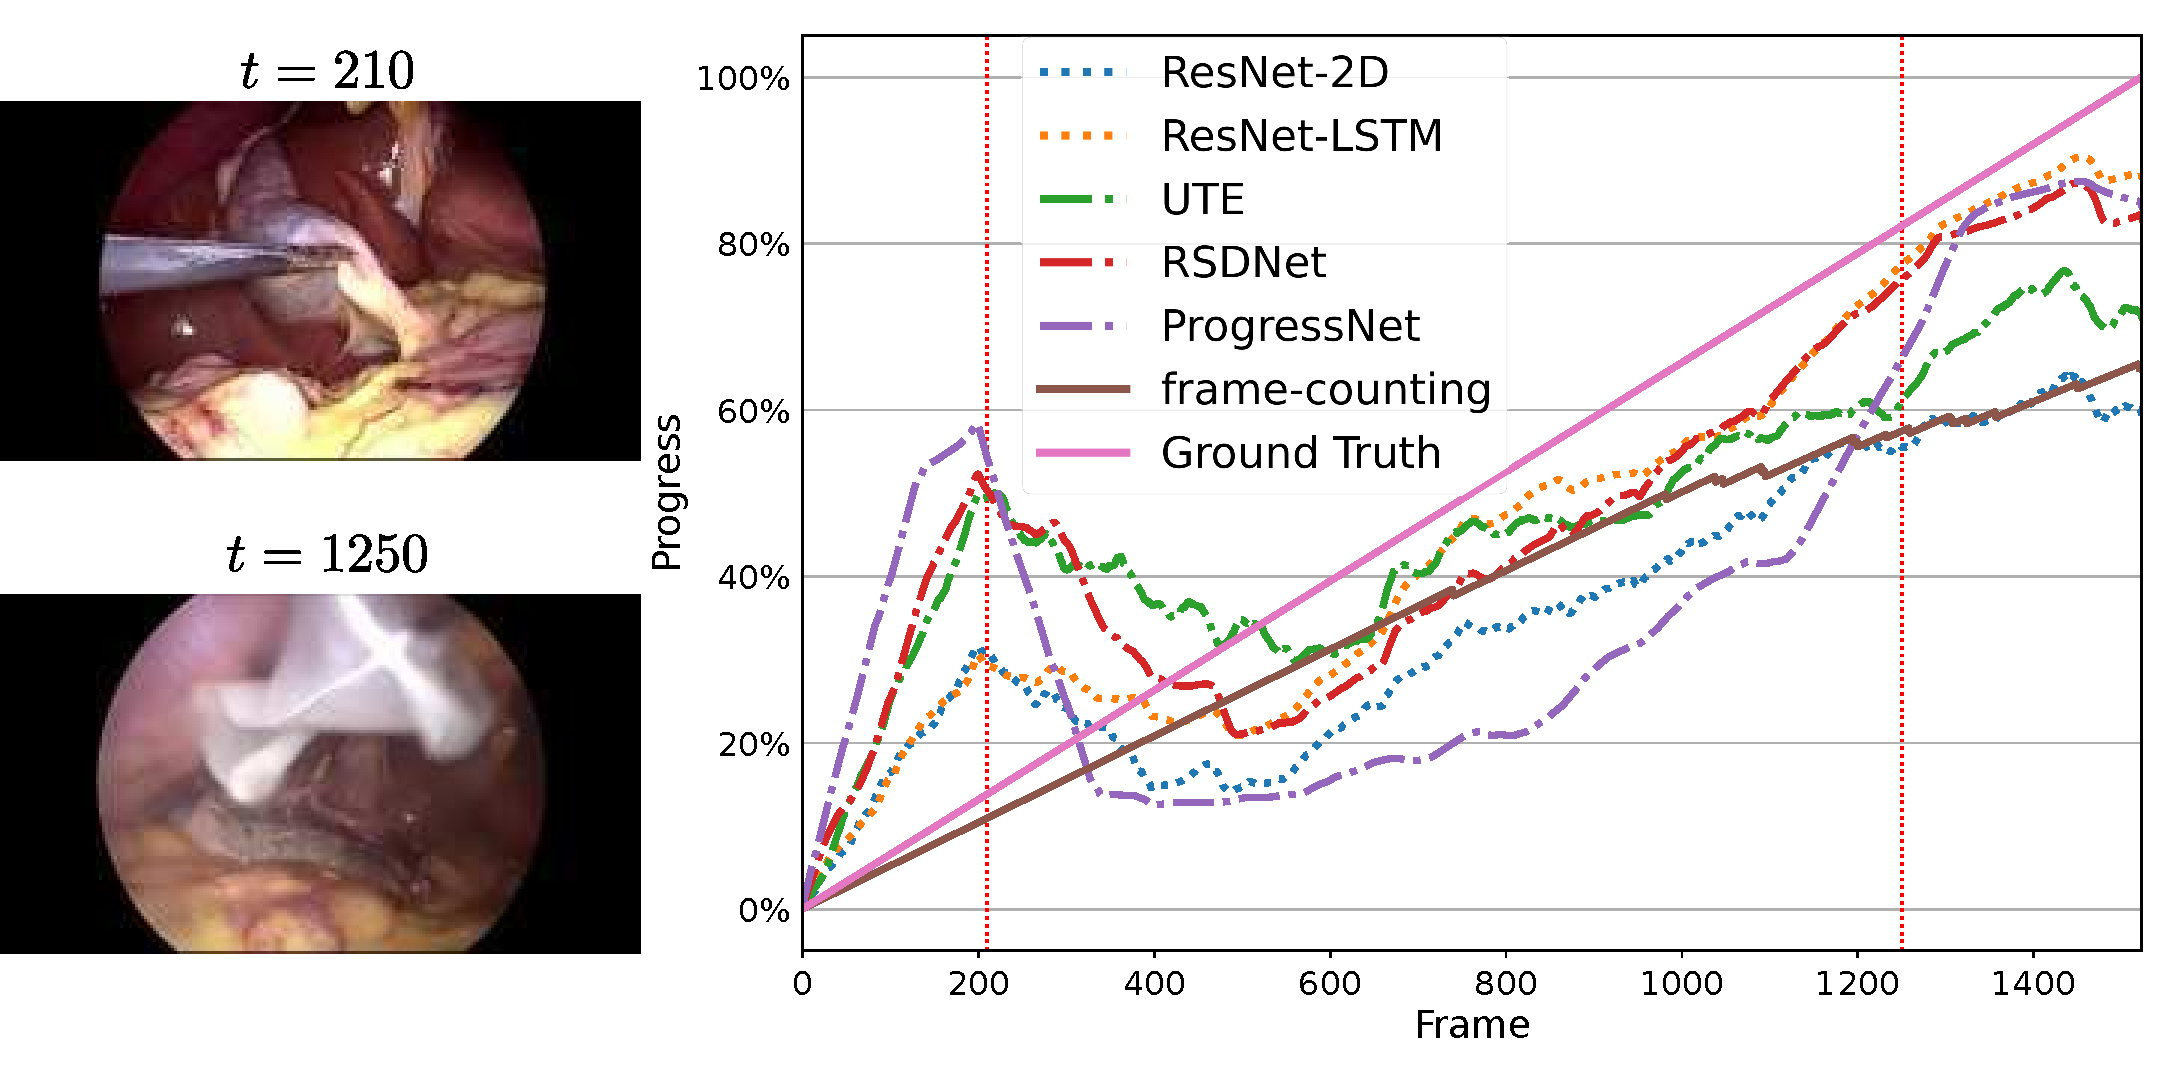
\includegraphics[width=.45\linewidth]{media/examples/cholec_ex2.pdf}
    & 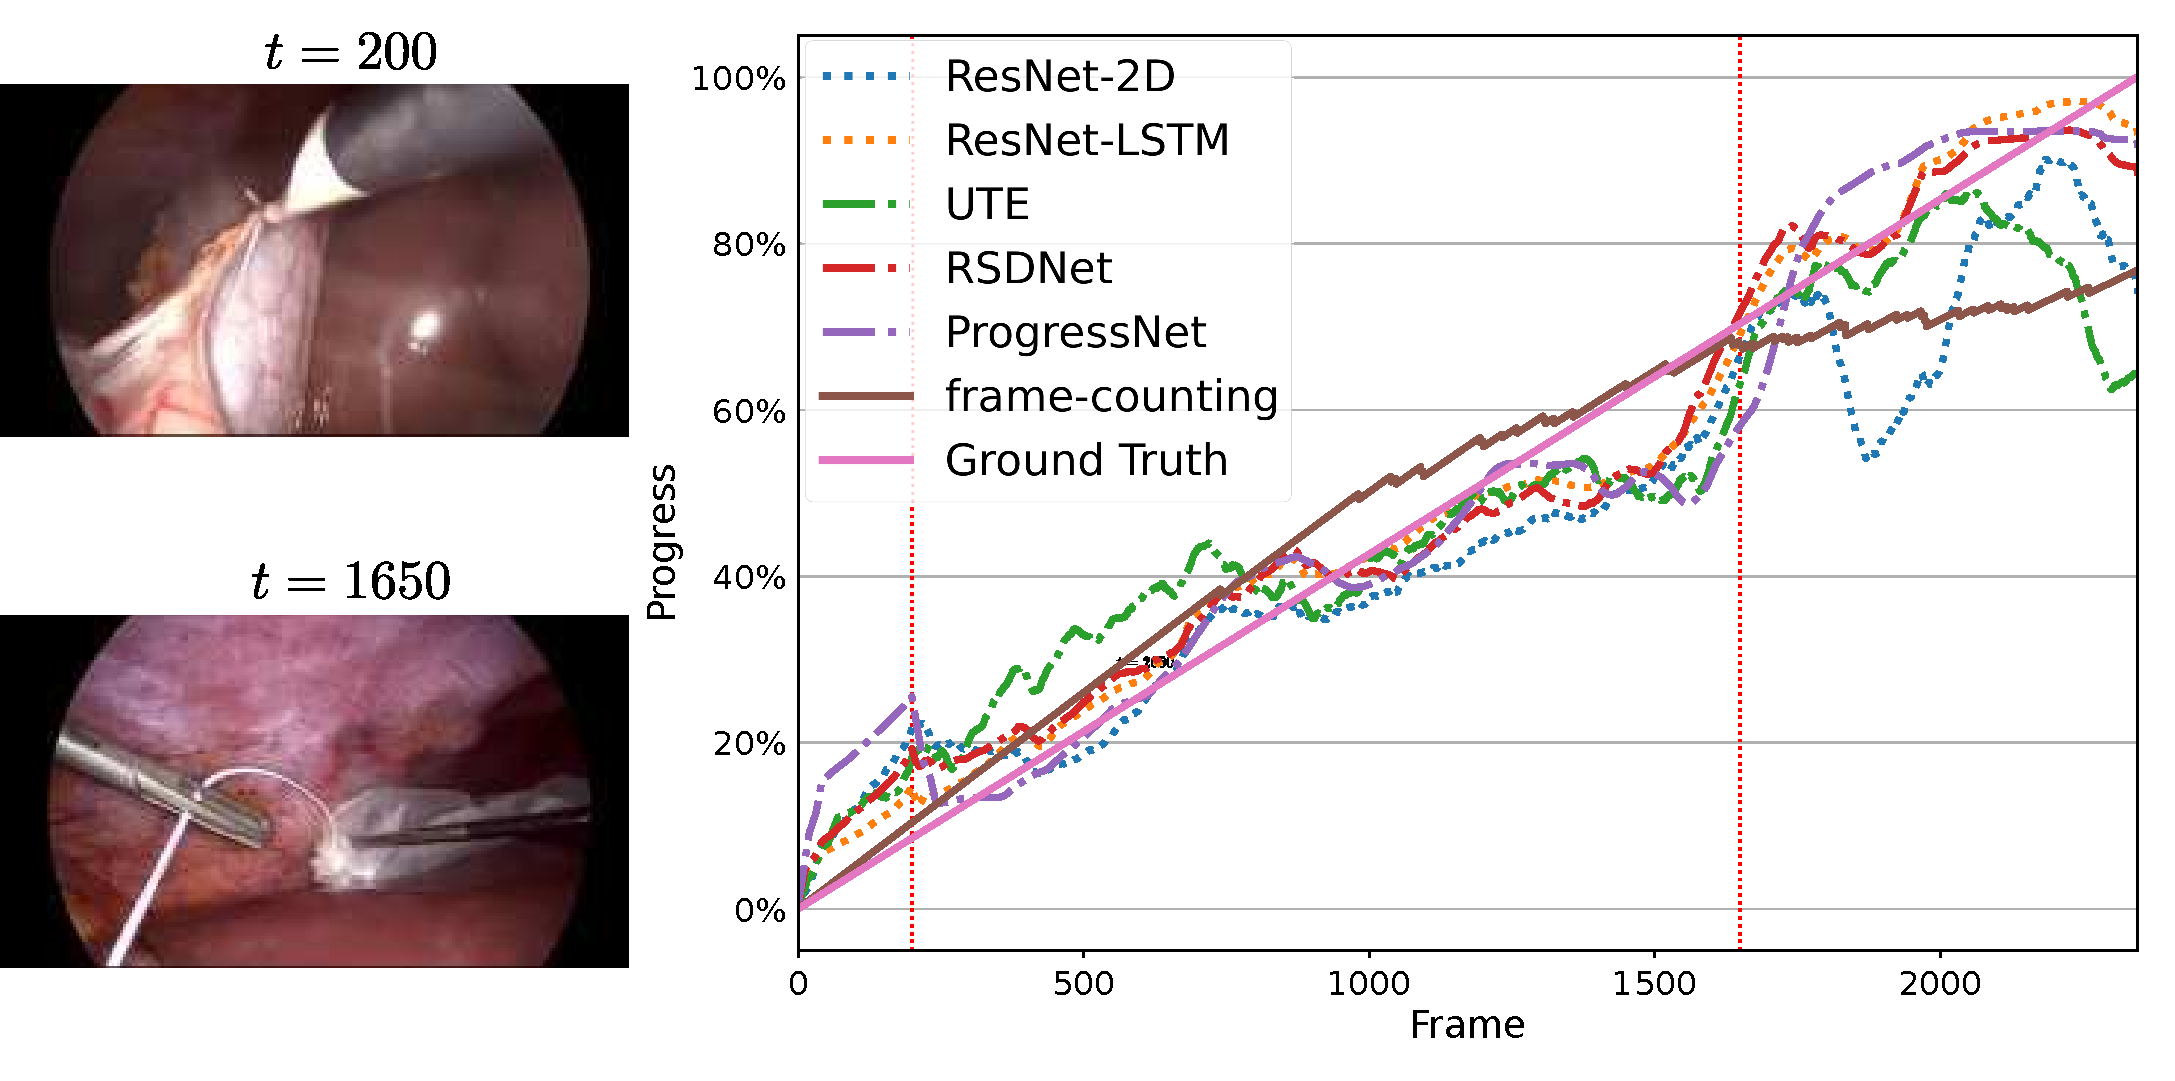
\includegraphics[width=.45\linewidth]{media/examples/cholec_ex1.pdf} \\
    {\small (a) Video-04 of \textsl{Cholec80}} & 
    {\small (b) Video-05 of \textsl{Cholec80}} \\
    \end{tabular}
\end{center}
   \caption{Activity progress prediction examples of \textsl{Cholec80}.
   (a) Video-04 at timestamps $t{=}210$ and $t{=}1250$. 
   (b) Video-05 at timestamps $t{=}200$ and $t{=}1650$. 
    At $t{=}210$ and $t{=}200$ the methods recognize the medical tool, and correct their progress downwards to signal the start of the medical procedure.
    At $t{=}1250$ and $t{=}1650$ the methods recognize the collection bag and correct their progress to signal the end of the procedure.}
\label{fig:cholec_videos}
\end{figure*}

\begin{figure}
\begin{center}
    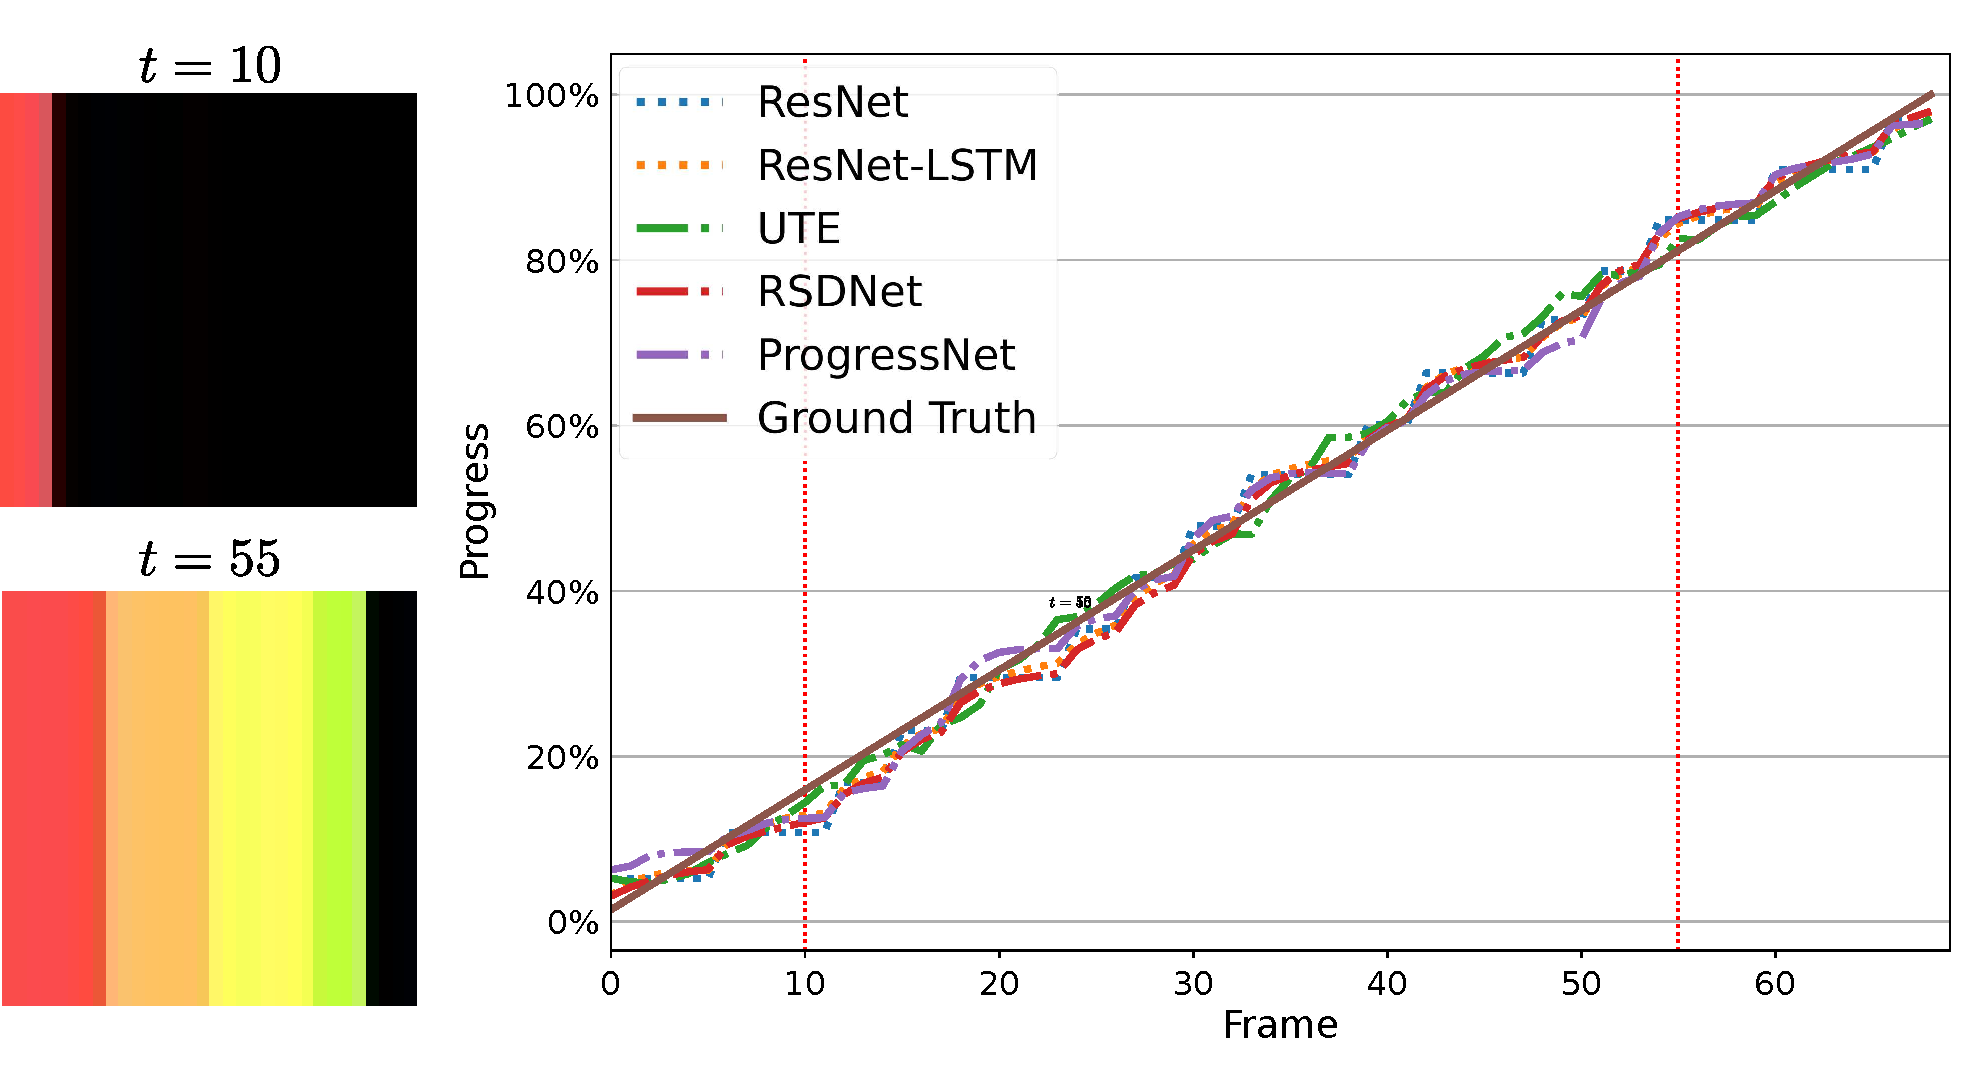
\includegraphics[width=1.0\linewidth]{media/examples/bar_ex1.pdf} 
\end{center}
   \caption{Progress prediction example on Video-00015 of our synthetic \textsl{Progress-bar} dataset at timestamps $t{=}10$ and $t{=}55$. 
   The learning methods can almost perfectly follow the ground truth.}
\label{fig:bars_00015}
\end{figure}

\noindent\textbf{Discussion.} 
This paper empirically shows that the current progress prediction datasets do now allow for learning useful visual information, and methods are outperformed by naive baselines relying on dataset statistics. 
However, we also saw that some visual information was learned on the \textsl{Cholec80}.
This may be due to the presence of clear visual phase delineators. 
\fig{cholec_videos}(a) and \fig{cholec_videos}(b) show examples of predictions on the \textsl{Cholec80} dataset. 
The first frames highlighted in these videos ($t{=}210$ and $t{=}200$) are the moment when the first medical tool is present in the video, and the progress prediction methods adjust their predictions to this new visual information. 
Similarly, the second highlighted timesteps ($t{=}1250$ and $t{=}1650$) represent the moment the collection bag is present which signals the end of the procedure. 
On our synthetic \textsl{Progress-bar} dataset in \fig{bars_00015} we also show the predictions and highlight two moments in the videos. 
Here, the networks almost perfectly follow the ground truth progression. 
These results illustrate that for progress prediction is essential to have clearly recognizable visual transition points, that consistently correspond to a certain progress prediction percentage. 
This is related to the idea of Becattini \etal \cite{becattini2017} who use phase annotations to increase the loss around the phase boundaries.

\smallskip\noindent\textbf{Limitations.} 
The first limitation of our research is that we could only find 3 progress prediction methods to analyze, on 3 datasets. 
Additionally, we do not consider here other video-architectures such as a Video Transformer \cite{arnab2021}, as these are not directly related to the progress prediction methods we analyze.
However, we do consider 2D (ResNet) and 3D (I3D) convolutional embeddings, as well as recurrent networks (with LSTM blocks). 
Thirdly, we were unable to match the results of \textsl{ProgressNet} exactly as reported in \cite{becattini2017}: 
when trained on \textsl{video-segments}, the authors report an MSE of $0.052$ (MAE of approximately $22.8$\%), while we obtain an MAE of $25.9$\%.
Nonetheless, the \textsl{frame-counting} outperforms the result reported in \cite{becattini2017}, which still validates our conclusions.
Finally, we observed that on both \textsl{UCF101-24} and \textsl{Breakfast} the methods have a tendency to overfit. 
Maybe better strategies to overcome this overfitting phenomenon could improve the results.

